%---=---==---===---====---=====---======---=====---====---===---==---=---%
%-                             INTRODUCTION                             -%
%---=---==---===---====---=====---======---=====---====---===---==---=---%

\chapter{Introduction}\label{chap:introduction}
\pagenumbering{arabic}

This introduction serves to give an insight into, and the \nameandsecref{sec:motivation} of, the \nameandsecref{sec:problem} that this paper aims to solve, and also present some \nameandsecref{sec:challenges} that are expected to be faced throughout.

\section{Motivation}\label{sec:motivation}

Augmented reality (AR) can be thought of as lying on \possessivecite{rvcontinuum} Reality-Virtuality (RV) continuum (\cref{fig:continuum}), which defines the transition between an environment consisting solely of real objects, and an environment consisting solely of virtual objects.  AR lies close to the real environment on the RV continuum, more specifically AR is the addition of virtual objects onto real objects. When discussing AR, people are usually referring to visual AR, however it is worth noting that can potentially apply to all senses, including hearing, touch, and smell \citep{aradvances}.

\begin{figure}[ht]
    \centering
    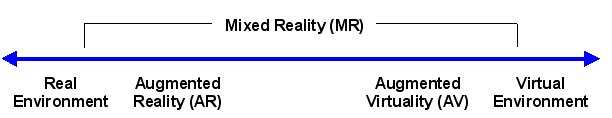
\includegraphics[width=0.8\textwidth]{images/proposal/RealityVirtualityContinuum}
    \caption{Simplified representation of a RV Continuum \protect\citep{rvcontinuum}.}
    \label{fig:continuum}
\end{figure}

Visual AR systems can be viewed through the use of projection displays, hand-held displays and head-worn displays. Some examples of head-worn displays currently in the market are shown in \cref{fig:headworndisplays}: Microsoft HoloLens, used for gaming and everyday applications such as video calling; Epson Moverio BT-300FPV Drone Edition, used for controlling a remote drone; and Google Glass Enterprise Edition, used to help businesses for activities like factory work and surgery. Smartphones and tablets can be used as hand-held displays, and are widely available as there are currently a predicted 2.53 billion smartphone users worldwide \citep{emarketer}. Uses for hand-held displays stretch from gaming and entertainment to training and education.

AR has recently gained popularity across many disciplines, and is estimated to explode in the coming years, as shown in \cref{fig:arstats}. A most notable area in AR is gaming, in which an AR smartphone game, Pokemon Go, hit a daily user count of 45 million, mere days after its release \citep{pokemongo}; an incredible achievement which was made possible through the use of new AR technology. It follows from these statistics that there is significant market potential in AR, specifically for AR in gaming.

\begin{figure}[ht]
\begin{minipage}{\textwidth}
\centering
\begin{minipage}{0.3\textwidth}
    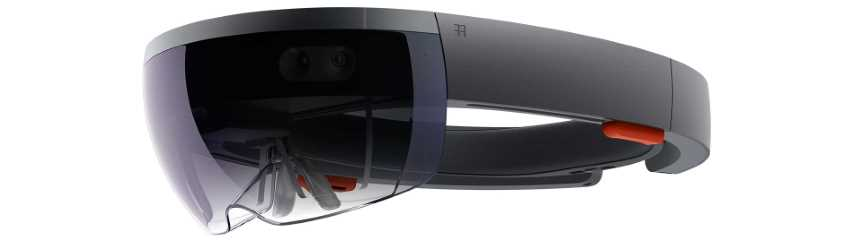
\includegraphics[width=\textwidth]{images/proposal/microsoft-hololens}
    \label{fig:hololens}
\end{minipage}\hfill
\begin{minipage}{0.3\textwidth}
    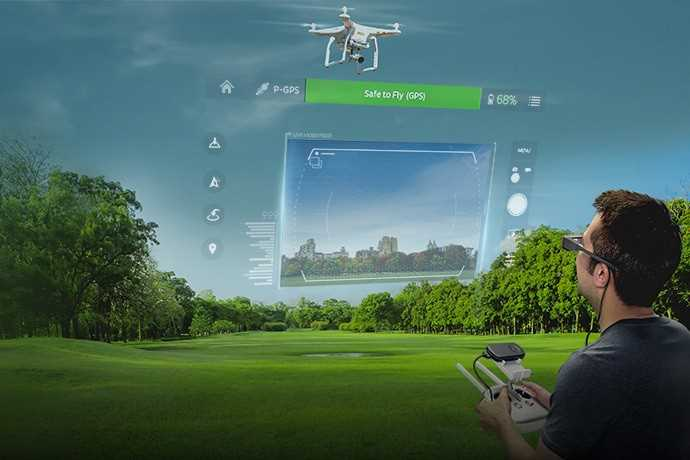
\includegraphics[width=\textwidth]{images/proposal/moverio-smart-glasses-2}
    \label{fig:epson}
\end{minipage}\hfill
\begin{minipage}{0.3\textwidth}
    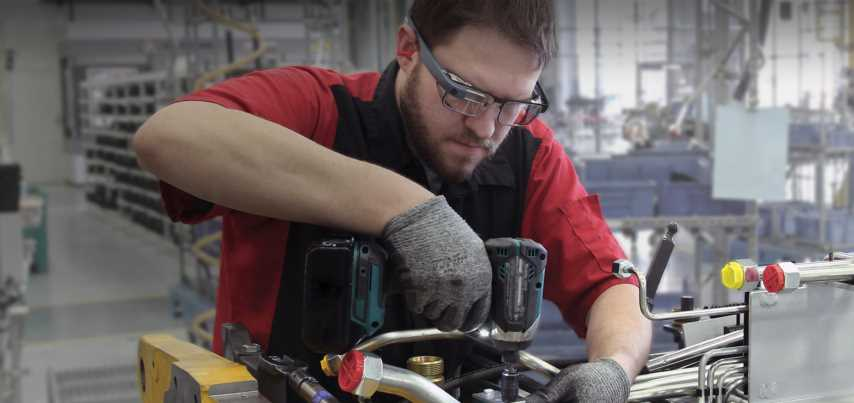
\includegraphics[width=\textwidth]{images/proposal/google-glass}
     \label{fig:glassee}
\end{minipage}
\caption{Current head-worn displays. \protect\footurl{https://www.microsoft.com/en-us/hololens}{Microsoft HoloLens} (left), \protect\footurl{https://epson.com/For-Home/Smart-Glasses/Smart-Glasses/Moverio-BT-300FPV-Smart-Glasses-\%28FPV-Drone-Edition\%29/p/V11H756020F}{Epson Moverio BT-300FPV Drone Edition} (centre), and \protect\footurl{https://x.company/glass/}{Google Glass} (right).}
\label{fig:headworndisplays}
\end{minipage}
\end{figure}

\begin{figure}[ht]
    \centering
    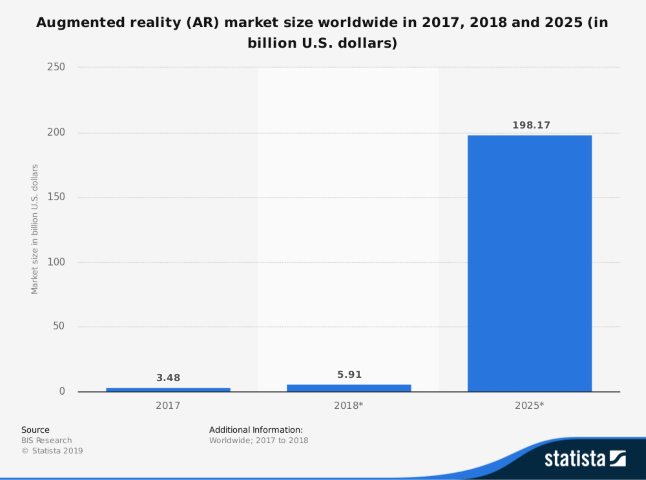
\includegraphics[width=0.65\linewidth]{images/proposal/statistic_id897587_augmented-reality-market-size-worldwide-2017-2025}
    \caption{Augmented reality (AR) market size worldwide in 2017, 2018 and 2025 (in billion U.S. dollars) \protect\citep{bisresearch}}
    \label{fig:arstats}
\end{figure}


%%
%
\section{Problem}\label{sec:problem}
%
%%

\jenga{} is a physical skill game that comprises of 54 wooden blocks, which begin, in a starting state, stacked in a tower of 3 block wide layers, with layers alternating between a 0\degree{} and 90\degree{} orientation. Players take turns in removing a block from the tower, and then placing that block on top of the tower, all whilst trying to prevent the tower from toppling over.

\begin{figure}[ht]
\begin{minipage}{\textwidth}
    \centering
    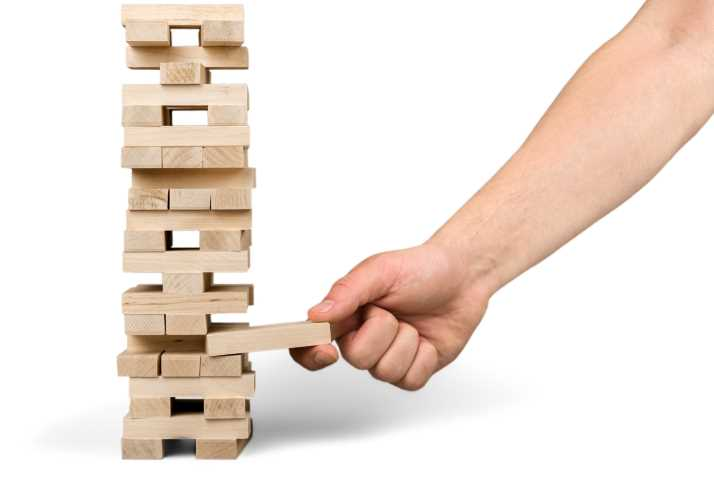
\includegraphics[width=0.5\linewidth]{images/proposal/jenga.jpeg}
    \caption{A \jenga{} tower obtained from \protect\footurl{https://stock.adobe.com/uk/}{Adobe Stock}}
    \label{fig:jenga}
\end{minipage}
\end{figure}

The main problem faced by players of \jenga{} is choosing which block to remove. Some variants even prevent the player from touching multiple blocks during their turn, thus they need to make a good decision before attempting block removal. Reasons to consider when deciding on the feasibility of removing a block depends on its situation in the tower, and can include: the block is supporting the structure above it, weighing down one side of the tower, is the last remaining in its layer, or is not easily accessible.

Several papers have addressed the aforementioned problem, some of which are discussed later in the \nameandsecref{chap:background}. However, current solutions rely on a fixed position camera, using a tripod, which would not be applicable in real instances of the game because players rarely have access to such camera equipment. In addition, previous projects which utilise the growing AR technology have all done so by creating a fully virtual tower in the starting state and adding that to the real environment. Furthermore, previous work done in the area also assume certain properties, such as alternating odd-even rows, and that blocks will be aligned to the shape of the tower.

This paper proposes a solution to the problem that allows for a more readily available free-moving camera, such as a smartphone. It also aims to make use of a real-world \jenga{} tower, which can be in any game state, meaning any number of player turns could have occurred before the system is first used, and also that individual blocks can be in any rotational or translational state. Doing this would improve significantly on the state-of-the-art technologies and research in the area.

The project spans over three crucial stages: firstly the detection of block poses, then an analysis of block removal feasibility, and finally result visualisation. In many sections of the report, it is deemed appropriate to treat the stages as separate entities that communicate by passing information between each other, and as such, the sections will retain a degree of modularity within this regard.

\section{Challenges} \label{sec:challenges}

Some challenges that may be faced in the undertaking of this project are detailed in the sections below:

As the solution aims to use real cameras, problems could arise due to the properties of each camera, such as image size and distortion. For example, if a camera is not calibrated to address distortion, then estimations of pose could be extremely inaccurate.

When using the system there may be times when the tower is not in-frame (visible by the camera), which could cause issues with false-positive detection. Furthermore, it may be difficult for the system to be able to distinguish between a block and a non-block gap in the tower because computer vision techniques need to be applied carefully to work well.

Reconstructing the tower for analysis may prove challenging as there may be inaccuracies in the detection of the blocks, as pose cannot be known, only estimated. In addition, finding a good method to analyse the block removal feasibility will be tough because accurately analysing real world physics is still an area of ongoing research in computer science.

Finally, as there are several ways to implement augmented reality in applications today, making it a troubling task to choose the right tool for displaying the results to the user.
Another item that needs to be considered is the creation of the user interface, with which ensuring usability is far from straightforward.

\section{Objectives}\label{objectives}

There are 3 objectives to work towards in this project, if all three objectives are met then the system is complete to the intended standard:

\begin{enumerate}
    \item\label{obj:detect} \textbf{Detect the poses of blocks in a real tower}
    \item\label{obj:analysis} \textbf{Analyse the removal feasibility of each block}
    \item\label{obj:display} \textbf{Visualise the results in an aesthetically pleasing manner}
\end{enumerate}

These objectives will be evaluated later on with a discussion into why they were, or indeed were not met by the end of the project.

Following this introduction, the paper will include; a \nameandsecref{chap:background} of the technologies used, capturing and setting project \nameandsecref{chap:requirements}, detailed \nameandsecref{chap:design} and \nameandsecref{chap:implementation}, all followed by a comprehensive \nameandsecref{chap:evaluation} and some thorough \nameandsecref{chap:conclusions}.



